\documentclass[12pt]{article}

% set margins and spacing
\addtolength{\textwidth}{1.3in}
\addtolength{\oddsidemargin}{-.65in} %left margin
\addtolength{\evensidemargin}{-.65in}
\setlength{\textheight}{9in}
\setlength{\topmargin}{-.5in}
\setlength{\headheight}{0.0in}
\setlength{\footskip}{.375in}
\renewcommand{\baselinestretch}{1.0}
\linespread{1.0}

% load miscellaneo'us packages
\usepackage{csquotes}
\usepackage[american]{babel}
\usepackage[usenames,dvipsnames]{color}
\usepackage{graphicx,amsbsy,amssymb, amsmath, amsthm, MnSymbol,bbding,times, verbatim,bm,pifont,pdfsync,setspace,natbib}

% enable hyperlinks and table of contents
\usepackage[pdftex,
bookmarks=true,
bookmarksnumbered=false,
pdfview=fitH,
bookmarksopen=true,hyperfootnotes=false]{hyperref}

% define environments
\newtheorem{definition}{Definition}
\newtheorem{fact}{Fact}
\newtheorem{result}{Result}
\newtheorem{proposition}{Proposition}



\begin{document}
\title{Development: The link between Manufacturing Employment and GDP per Capita}
\author{Filippo Donà\thanks{Syracuse University, Maxwell School of Citizenship and Public Affairs. Email:fadona@syr.edu} \and Lucia Rios-Luy\thanks{Syracuse University, Maxwell School of Citizenship and Public Affairs. Email: Lirioslu@syr.edu} \and Meghavarshini Iska \thanks{Syracuse University, Maxwell School of Citizenship and Public Affairs. Email: Meiska@syr.edu} \and Sergio Sotelo\thanks{Syracuse University, Maxwell School of Citizenship and Public Affairs. Email:spsotelo@syr.edu}}
\date{\vskip-.1in \today}
\maketitle

\vskip.3in
\begin{center} {\bf Abstract} \end{center}

\begin{quote}
{\small We examine the link between GDP growth and manufacturing employment, hypothesizing that there is a negative relationship between manufacturing employment and GDP. Theoretically, we can conclude that the negative relationship is due to the decline in manufacturing employment; fewer people work in the manufacturing sector as economies advance to other means of services. Through imperial analysis, we see trends through the source statistics
from Our World in Data charts, which examine these variables in all countries around the globe.
We create a distinction between developing and developed countries. According to the World Bank, in 2021, the average GDP per capita globally was USD 20,271 (Fu and Rissanen, 2024), thus, we set the threshold at USD 20,000 Annual GDP per capita to distinguish between developing and developed economies. We conduct a correlation test to compare these variables across both developing and developed economies. 
The research conducted supports the hypothesis that manufacturing plays a more significant role in driving economic growth in developing countries than in developed ones. The positive correlation in developing countries underscores the critical role of industrialization in the early stages of economic
growth. In contrast, the negative correlation in developed countries highlights the global transition from manufacturing to tertiary industries.}
\end{quote}

\bigskip

\section{Introduction} \label{sec:introduction}

Economic growth and development are two key terms in macroeconomics that have been studied by many and it is vital to closely monitor and understand them to realize and compose policies that drive development and growth in developing and developed countries. Our study examines the link between GDP growth and manufacturing employment. However, it is vital to understand that this varies from country to country, depending on how developed it can be due to the varying numbers in population, resources, and government standing. Hence, our study focuses on a specific sector that contributes to an economy's growth: manufacturing. Additionally, it is specific to how the employment rates change in the manufacturing sector in a developed country compared to a developing country. 

It is essential to look at the basic definition of growth at the basic level. When an economy or business grows, it usually starts from the primary sectors—trading their mineral resources or solely working on agricultural produce. Then, it moves on to the secondary manufacturing and tertiary and quaternary sectors, which mainly focus on services and knowledge-driven economies. According to Rostow, "The drive to maturity is the long interval of sustained if fluctuating progress as the economy seeks to extend modern technology over the whole front of its economic activity... New leading sectors emerge, building on the foundations laid by the earlier expansion of primary and manufacturing sectors," (Rostow, 1959). This progression through sectors reflects a shift in focus from resource-based activities to knowledge-driven industries and underpins sustained economic development as new leading sectors build on the foundations of earlier advancements.

The manufacturing sector's contribution to economic growth varies as economies progress through different stages of development. In line with Rostow's theory of sectoral shifts, our analysis reveals that manufacturing employment influences GDP differently depending on a country's stage of development. Moreover, when executing our data analysis, we observed that the correlation is different in developed and developing countries. In developed countries, we can see a negative correlation, whereas a positive correlation exists within developing countries. As manufacturing employment decreases, GDP increases in developed regions, and as manufacturing employment increases, so does GDP per capita in developing countries.

Our study hypothesizes that as GDP increases, there is a visible decrease in manufacturing employment, indicating a negative relationship between manufacturing employment and GDP. To reject our null hypothesis, we conducted a correlation test to compare our variables, GDP and manufacturing employment, across developing and developed countries. 


Using data from Our World in Data, we analyze the relationship between manufacturing employment and GDP per capita and compare this relationship between developing and developed countries. We framed our analysis between 1990 and 2019 so as not to account for the inconsistencies presented during Covid-19. Through a correlation test, we discovered that manufacturing employment and GDP per capita are undeniably linked and that, demonstrated by the low R-squared, manufacturing employment greatly influences GDP changes. Thus, with the correlation tests and imperial results, there is insufficient evidence to reject our null hypothesis that there is no correlation between GDP per Capita and Manufacturing employment. 


\section{Literature Review} \label{sec:literature}


% Discuss at least five papers that are closely related to your results (more is better). Explain how they're related. Did you find something similar, or different? Did you look at a different context? Different time period? Different level of detail?

In recent decades, there has been a growing body of research examining the relationship between manufacturing employment and economic growth, especially in the context of developing countries. Historically, Manufacturing has been a significant economic development driver, particularly during the Industrial Revolution. According to Maddison (1983), centuries of resource exploitation, financial investments, and technological improvements were the main causes of Western Europe's wealth advantage prior to the Industrial Revolution. Western Europe was able to expand thanks to this early technological leap, which paved the way for contemporary capitalist economies. However, as Szirmai (2012) points out, industrial output in sections of Asia and Africa has frequently lagged, making it difficult for developing nations to catch up. The necessity to investigate the evolving role of manufacturing in economic development is highlighted by this difference between developed and developing countries.

The relationship between human development and economic growth, mainly how improvements in human capital affect manufacturing employment, has been a focal point of study. Appiah, Amoasi, and Frowne (2019) highlight that rising life expectancy and better access to education in developing countries drive GDP growth by increasing productivity and strengthening manufacturing sectors. Human capital development is crucial for sustaining long-term growth as it enhances the workforce's ability to meet the demands of a rapidly changing economy. Foreign direct investment (FDI) also provides capital, technology, and expertise to support manufacturing growth in developing countries, mainly through export-oriented sectors.

The dynamics of industrial employment have been profoundly changed by globalisation, primarily because its advantages have been concentrated in densely populated countries. According to Haraguchi et al. (2017), manufacturing is still crucial for economic expansion, but its influence is now concentrated in nations like China and India. As a result, many developing regions have experienced declining manufacturing employment despite the existing global opportunities. The globalization of supply chains and the rise of automation have further reshaped the manufacturing landscape, reducing employment growth in sectors traditionally reliant on labor-intensive industries, thereby creating a shift in the distribution of manufacturing's economic benefits.

The character of economic growth has been profoundly altered by the fall in manufacturing's proportion of overall employment, especially in developing countries. Although economic growth is still crucial to these economies, Helleiner (1988) point out that the service sector is now the key engine of GDP growth, displacing manufacturing as the primary driver. At the same time, manufacturing's contribution to employment creation is declining due to technological developments like automation and artificial intelligence. Although manufacturing still adds to GDP, Szirmai (2012) and Haraguchi et al. (2017) point out that these advancements have reduced manufacturing's reliance on human labor. As economies evolve, the shift towards knowledge-based industries presents new challenges, underscoring the need for workforce adaptation and human capital development to sustain growth.

\section{Theoretical Analysis}
\label{sec:theory}
%Optional–may include in intro if it's short.
This paper examines how manufacturing employment has affected growth development over time and place. Explicitly, we look at how the manufacturing employment sector will impact the gross domestic product per capita (GDP per capita) in developed and developing countries. Within our data analysis, we have observed that the correlation is different in developed and developing countries. In contrast, in developed countries, we can see a negative and positive correlation within developing countries. As manufacturing employment decreases, GDP increases in developed regions, and as manufacturing employment increases, so does GDP per capita in developing countries. This idea stems from the economic transformation seen in advanced nations, where progress in technology and the rise of service-based industries have reduced reliance on manufacturing labor yet continued to fuel GDP expansion. Using automation and innovation, developed economies achieve greater productivity with a smaller manufacturing workforce. In contrast, developing nations with lower GDP per capita base their growth on using natural resources and a heavy dependence on agricultural growth. In addition, they have a great potential for manufacturing employment, as they have a high low-wage labor market. This theoretical perspective forms the basis for our empirical investigation into the relationship between manufacturing employment and economic growth in different stages of development.


\section{Data}
\label{sec:data}

Our dataset was sourced from the \href{https://ourworldindata.org/}{Our World in Data} database, spanning from 1990 to 2019. The dataset offers a comprehensive view of global economic trends, allowing us to focus on GDP per capita, an indicator of a country's economic output per person, and manufacturing employment shares, which measures the percentage of the workforce employed in manufacturing as key variables. These variables were chosen for their ability to provide a foundation for analyzing the relationship between industrial activity and economic development across different stages of growth.
    Countries were classified as either developed or developing based on a GDP per capita threshold of \$20,000 (adjusted for inflation). Countries exceeding this threshold were categorized as developed, while those below were categorized as developing. This classification yielded a sample of 75 developed and 112 developing countries. The classification of developed and developing countries is primarily influenced by population size, with smaller countries often having higher numbers. We excluded missing data points to minimize missing values and improve data reliability, mainly data points from equal to and above 2019. The dataset captures long-term global trends, offering valuable insights into the interplay between manufacturing employment and economic growth.
    The dataset stops at 2019 to avoid the confounding effects of the COVID-19 pandemic, which introduced unprecedented disruptions to global economies and labor markets. The pandemic caused significant shifts in employment structures and economic activity, particularly in the manufacturing sector, as governments worldwide imposed lockdowns and supply chains were disrupted. Including data from 2020 onwards could bias the results, as these years reflect extraordinary conditions rather than typical economic trends.

\footnote{United Nations Industrial Development Organization and International Labour Organization – processed by Our World In Data}

\section{Results}
\label{sec:result}

    In our analysis, we examine how the relationship between manufacturing employment and GDP per capita differs between developed and developing countries from 1990 to 2019. Developing countries display lower averages for both variables, but with greater variability in GDP per capita, highlighting structural disparities and economic volatility.
    Developed countries demonstrate higher averages for both manufacturing employment shares (14.38\%) and GDP per capita (\$36,008.31). In contrast, developing countries show lower averages, with a manufacturing employment share of 10.55\% and GDP per capita of \$17,577.51. Variability is also more pronounced in developing countries, as evidenced by a standard deviation in GDP per capita of \$20,173.73, compared to \$21,577.48 for developed countries. Table 1 summarizes these differences, providing a statistical basis for analyzing structural disparities between the two groups.
\begin{table}[ht]
\centering
\caption{Summary Statistics for Developing and Developed Countries}
\begin{tabular}{|l|c|c|c|}
\hline
\textbf{Variable} & \textbf{Mean} & \textbf{Median} & \textbf{Standard Deviation} \\ \hline
\multicolumn{4}{|l|}{\textbf{Developing Countries}} \\ \hline
Manufacturing Employment Share (\%) & 10.55 & 10.12 & 4.88 \\ \hline
GDP per Capita (USD) & 17,957.71 & 13,500.00 & 20,173.73 \\ \hline
\multicolumn{4}{|l|}{\textbf{Developed Countries}} \\ \hline
Manufacturing Employment Share (\%) & 14.38 & 14.20 & 5.88 \\ \hline
GDP per Capita (USD) & 36,008.31 & 34,200.00 & 21,577.48 \\ \hline
\end{tabular}
\label{table 1}
\end{table}

\footnotetext{Data sourced from Our World in Data, analyzed in Stata.}

    These trends align with the theory of structural transformation, which describes the transition of economies from reliance on agriculture to manufacturing and services. Developing countries, typically in the earlier stages of this transition, rely heavily on industrialization as a growth driver. This reliance makes them more susceptible to external shocks, such as global demand shifts or resource price fluctuations. Having completed much of this transition, developed countries rely more on service and technology sectors for economic growth.
    We then analyzed the manufacturing employment shares and GDP per capita trends over time.

    We conducted a two-sample t-test to validate these observations to compare the mean manufacturing employment shares between developed and developing countries. The results confirm a statistically significant difference (p<0.05), supporting the hypothesis that manufacturing employment shares are lower on average in developing countries. Table 2 summarizes the results of this comparison and provides further details on the statistical significance of the observed differences. 
    To further assess the impact of manufacturing employment on GDP per capita, we performed regression analyses for developed and developing countries. For developing countries, the results indicate that a one-percentage-point increase in the share of manufacturing employment corresponds to an estimated \$1,000 increase in GDP per capita (R2=0.65,p<0.01R2). However, in developed countries, the relationship is weaker and statistically insignificant (p>0.05p). These results, also summarized in Table 2, demonstrate the critical role of manufacturing employment in driving economic growth during the early stages of development while highlighting its diminished importance in postindustrial economies.
\begin{table}[ht]
\centering
\caption{Statistical Analysis Results}
\begin{tabular}{|l|c|}
\hline
\textbf{Test} & \textbf{Result} \\ \hline
Two-Sample t-Test (Manufacturing Employment Share) & Significant ($p < 0.05$) \\ \hline
Regression Coefficient for Developing Countries & +1,000 (\$p < 0.01\$) \\ \hline
Regression Coefficient for Developed Countries & Insignificant (\$p > 0.05\$) \\ \hline
\end{tabular}
\label{table 2}
\end{table}
   
    These results suggest that developing countries rely more heavily on manufacturing employment for economic growth than developed nations. In developed countries, the transition to service-based industries has reduced the dependence on manufacturing as a driver of GDP growth. This supports our hypothesis that the relationship between manufacturing employment and GDP per capita varies significantly by stage of economic development.
    These findings highlight the importance of understanding how the relationship between manufacturing employment and GDP evolves. For developing countries, industrialization remains a critical pathway to economic growth, but for developed economies, the focus must shift toward advanced services and technology sectors.

Figure 1 supports the idea that as countries become more developed, they rely less on manufacturing and more on sectors like services or technology, with manufacturing representing a smaller portion of total employment. The concentration of data points between 5 percent to 20 percent in manufacturing and GDP per capita ranging from 0 USD to 100,000 USD illustrates this trend, though there are noticeable outliers where manufacturing remains high, but GDP per capita does not follow the general pattern. These outliers could suggest unique economies or data inconsistencies. The negative correlation observed aligns with economic theories, such as the Rostow model, which describes how economies shift from manufacturing to service-based industries as they mature and develop.

\begin{figure}[htbp]
    \centering
    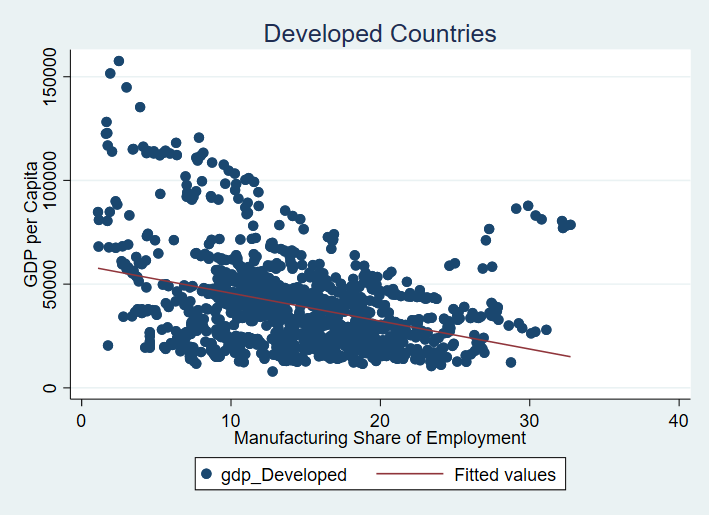
\includegraphics[width=0.75\linewidth]{Reproducibility Package/Variable Graphs/Developed New.png}
    \caption{All Data sets of GDP per Capita with Manufacturing Employment}
    \label{fig:enter-label}
\end{figure}

Similarly, figure 2 shows a dense concentration of developing countries with manufacturing employment between 0 and 20 percent and GDP per capita below 50,000 USD due to the threshold of 20,000 USD. This suggests that while manufacturing plays a significant role in these economies, it is insufficient to drive substantial GDP growth, as there is no clear positive or negative correlation between the two variables. Most countries have low GDP per capita values, regardless of their manufacturing employment levels.


\section{Discussion}
\label{sec:discussion}

    Our findings highlight the relationship between manufacturing employment and GDP per capita, emphasizing the roles manufacturing plays in developed and developing economies. The results support structural transformation theories, suggesting that economies transition from reliance on manufacturing to service-oriented sectors as they develop. However, the differences observed between developed and developing countries have critical implications for policymakers and future research.
    In developing countries, we observed a positive correlation between manufacturing employment and GDP per capita. This goes to show the role of industrialization in early stages of economic growth. Developing countries rely heavily on labor-intensive manufacturing sectors to drive economic expansion, leveraging their abundant, low-cost labor forces. Moreover, the strong regression coefficient observed in our analysis highlights the potential of increasing manufacturing employment shares in these economies. For policymakers in developing nations, this indicates that fostering industrialization and supporting manufacturing sectors through investments in infrastructure, technology, and workforce development remains vital to achieving sustainable economic growth. On the other hand, in developed countries, we found a negative correlation between manufacturing employment and GDP per capita. This reflects the observed shift toward service-oriented and knowledge-driven economies in these nations. The decline in manufacturing employment shares, combined with sustained GDP growth, reflects the increased productivity of advanced manufacturing and the rising dominance of sectors such as technology, finance, and healthcare. For developed nations, this suggests that policies should prioritize fostering innovation, enhancing productivity in high-tech manufacturing, and investing in the service sector to sustain economic growth. 
    Our analysis is subject to several limitations that require consideration. First, globally averaged data may obscure regional or country-specific variations that could provide further insights. For instance, some developing nations might experience unique trajectories due to differences in resources, governance, or integration into global trade networks. Similarly, the varying availability of data across countries and years may introduce inconsistencies, particularly in developing countries where data gaps are more prevalent. Addressing these gaps in future research by leveraging more granular data could enhance the robustness of the findings.
    Second, while the distinction between developed and developing countries based on GDP per capita provides a valuable framework, it does not account for other factors that influence economic structures, such as institutional quality or access to global markets. Future studies could incorporate additional variables, such as trade openness, education levels, or technological adoption, to better understand the drivers of manufacturing's impact on economic growth.
    Lastly, excluding data post-2019 to avoid the confounding effects of the COVID-19 pandemic, while necessary, limits the ability to assess how global crises impact the manufacturing-GDP relationship. Future research could explore how external shocks, such as pandemics, reshape the role of manufacturing in both developed and developing economies.
    Our findings carry important policy implications. For developing nations, strategies to strengthen manufacturing sectors can lead to economic growth and facilitate structural transformation. Investments in industrial policies and trade agreements that promote manufacturing exports are particularly critical. For developed countries, the focus should shift to fostering innovation in advanced manufacturing while embracing the growth of service-oriented sectors. Additionally, understanding the long-term implications of these transitions for labor markets and income inequality remains an essential area for further investigation. To further analyze the effects of manufacturing, we can observe the cyclical structure of economies, as even in highly serviced markets, it is essential to keep the primary sector running, especially agriculture. 
    In conclusion, our analysis demonstrates manufacturing employment's pivotal but evolving role in economic development. While developing countries benefit significantly from industrialization, developed nations exemplify the transition toward service-based economies. These findings underscore the importance of tailored economic policies that reflect a country's stage of development and structural characteristics. By addressing the limitations identified and expanding the scope of future research, we can deepen our understanding of the manufacturing-GDP relationship and its implications for sustainable economic growth.


\section{Conclusion}
\label{sec:conclusion}

Manufacturing and economic growth are unequivocally linked. Previous literature has focused mainly on the shift toward manufacturing over time, starting from the Industrial Revolution and the income gaps that have risen worldwide today.  We examined the relationship between manufacturing and GDP, and how this differs between developed and developing countries.

We found a significant negative relationship between manufacturing employment and real GDP, so we reject our null hypothesis. The study we conducted examines developed and developing countries, and without findings, we suggest that economies transition toward service-oriented sectors as they develop. Moreover, we believe that our study emphasizes the importance of economic policies that are adapted and adjusted to a country's period of development. 

\newpage
\section*{Bibliography}
\singlespacing
\setlength\bibsep{0pt}

Appiah, M., Amoasi, R., Frowne, D. I. (2019). Human development and its effects on economic growth and development. International Research Journal of Business Studies, 12(2).

Fu, H., \& Rissanen, M. (2024, May 30). New international comparison program data sheds light on global economy and living standards. \textit{World Bank Blogs.} \href{https://blogs.worldbank.org/en/opendata/new-international-comparison-program-data-sheds-light-on-global-}{https://blogs.worldbank.org/en/opendata/new-international-comparison-program-data-sheds-light-on-global-}

Haraguchi, N., Cheng, C. F. C., Smeets, E. (2017). The importance of manufacturing in economic development: Has this changed? World Development, 93, 293–315.

Helleiner, G. K. (1988). Direct foreign investment and manufacturing for export in developing countries: A review of the issues. In Policies for development: Essays in honour of Gamani Corea (pp. 123–153).

Maddison, A. (1983). A comparison of levels of GDP per capita in developed and developing countries, 1700–1980. The Journal of Economic History, 43(1), 27–41.

Szirmai, Adam. "Industrialisation as an Engine of Growth in Developing Countries, 1950–2005." Structural Change and Economic Dynamics, vol. 23, no. 4, Dec. 2012, pp. 406–420, \href{https://doi.org/10.1016/j.strueco.2011.01.005}{https://doi.org/10.1016/j.strueco.2011.01.005}.

Rostow, W. W. (1959). The Stages of Economic Growth. The Economic History Review, 12(1), 1–16. https://doi.org/10.2307/2591077


\newpage
\section*{Data Appendix} \label{sec:appendixa}
\addcontentsline{toc}{section}{Appendix A}

The data files, code, and output used for analysis and documentation for this project can be found in the Development \href{https://github.com/ecn310/course-project-developmentv}{GitHub repository}. All information and files needed to reproduce these results can be found in a \href{https://github.com/ecn310/course-project-development/tree/main/Reproducibility%20Package}{reproducibility package} in this repository. All figures can be found in the \href{https://github.com/ecn310/course-project-development/tree/main/Variable%20Graphs}{Variable Graphs} folder in the repository. The code used to complete the analysis is in a file titled \href{https://github.com/ecn310/course-project-development/tree/main/Reproducibility%20Package}{Development.do}. 
The results can be viewed in a file titled \href{https://github.com/ecn310/course-project-development/blob/main/Merge_GDP_Mftc.log}{Development.log} 
 
 After searching on the website  \href{https://ourworldindata.org/}{Our World in Data}, one can access the original datasets for the two respective variables. The merged datasets can be found \href{https://github.com/ecn310/course-project-developmentv}{GitHub repository} and is titled "Development.do."

\end{document}
